
\documentclass[12pt]{beamer}
\usepackage{amsmath}
\usepackage{mathtools}
\usepackage{multimedia}
\usepackage{hyperref}


\usefonttheme{professionalfonts} % using non standard fonts for beamer
\usefonttheme{serif} % default family is serif
%\documentclass[12pt]{beamerthemeSam.sty}
\usepackage{epsf}
%\usepackage{pstricks}
%\usepackage[orientation=portrait,size=A4]{beamerposter}
\geometry{paperwidth=160mm,paperheight=120mm}
%DT favorite definitions
\def\LL{\left\langle}	% left angle bracket
\def\RR{\right\rangle}	% right angle bracket
\def\LP{\left(}		% left parenthesis
\def\RP{\right)}	% right parenthesis
\def\LB{\left\{}	% left curly bracket
\def\RB{\right\}}	% right curly bracket
\def\PAR#1#2{ {{\partial #1}\over{\partial #2}} }
\def\PARTWO#1#2{ {{\partial^2 #1}\over{\partial #2}^2} }
\def\PARTWOMIX#1#2#3{ {{\partial^2 #1}\over{\partial #2 \partial #3}} }

\def\rightpartial{{\overrightarrow\partial}}
\def\leftpartial{{\overleftarrow\partial}}
\def\diffpartial{\buildrel\leftrightarrow\over\partial}

\def\BC{\begin{center}}
\def\EC{\end{center}}
\def\BN{\begin{enumerate}}
\def\EN{\end{enumerate}}
\def\BI{\begin{itemize}}
\def\EI{\end{itemize}}
\def\BE{\begin{displaymath}}
\def\EE{\end{displaymath}}
\def\BEA{\begin{eqnarray*}}
\def\EEA{\end{eqnarray*}}
\def\BNEA{\begin{eqnarray}}
\def\ENEA{\end{eqnarray}}
\def\EL{\nonumber\\}

\newcommand{\etal}{{\it et al.}}
\newcommand{\gbeta}{6/g^2}
\newcommand{\la}[1]{\label{#1}}
\newcommand{\ie}{{\em i.e.\ }}
\newcommand{\eg}{{\em e.\,g.\ }}
\newcommand{\cf}{cf.\ }
\newcommand{\BS}{\bigskip}
\newcommand{\etc}{etc.\ }
\newcommand{\atantwo}{{\rm atan2}}
\newcommand{\Tr}{{\rm Tr}}
\newcommand{\dt}{\Delta t}
\newcommand{\op}{{\cal O}}
\newcommand{\msbar}{{\overline{\rm MS}}}
\def\chpt{\raise0.4ex\hbox{$\chi$}PT}
\def\schpt{S\raise0.4ex\hbox{$\chi$}PT}
\def\MeV{{\rm Me\!V}}
\def\GeV{{\rm Ge\!V}}

%AB: my color definitions
%\definecolor{mygarnet}{rgb}{0.445,0.184,0.215}
%\definecolor{mygold}{rgb}{0.848,0.848,0.098}
%\definecolor{myg2g}{rgb}{0.647,0.316,0.157}
\definecolor{A}{rgb}{1.0,0.3,0.3}
\definecolor{B}{rgb}{0.0,1.0,0.0}
\definecolor{C}{rgb}{1.0,1.0,0.0}
\definecolor{D}{rgb}{0.5,0.5,1.0}
\definecolor{E}{rgb}{0.7,0.7,0.7}
\definecolor{abtitlecolor}{rgb}{1.0,1.0,1.0}
\definecolor{absecondarycolor}{rgb}{0.0,0.416,0.804}
\definecolor{abprimarycolor}{rgb}{1.0,0.686,0.0}
\definecolor{Red}           {rgb}{1,0.4,0.4}
\definecolor{Yellow}           {rgb}{1,1,0.0}
\definecolor{Grey}          {cmyk}{.7,.7,.7,0}
\definecolor{Blue}          {cmyk}{1,1,0,0}
\definecolor{Green}         {cmyk}{1,0,1,0}
\definecolor{Brown}         {cmyk}{0,0.81,1,0.60}
\definecolor{Silver}        {rgb}{0.95,0.9,1.0}
\definecolor{Sky}           {rgb}{0.07,0.0,0.2}
\definecolor{Darkbrown}     {rgb}{0.4,0.3,0.2}
\definecolor{Black}         {rgb}{0.0,0.0,0.0}
\definecolor{40Gray}        {rgb}{0.4,0.4,0.5}
\usetheme{Madrid}


\setbeamercolor{normal text}{fg=Silver,bg=Sky}

%AB: redefinition of beamer colors
%\setbeamercolor{palette tertiary}{fg=white,bg=mygarnet}
%\setbeamercolor{palette secondary}{fg=white,bg=myg2g}
%\setbeamercolor{palette primary}{fg=black,bg=mygold}
\setbeamercolor{title}{fg=abtitlecolor}
\setbeamercolor{frametitle}{fg=abtitlecolor}
\setbeamercolor{palette tertiary}{fg=white,bg=Darkbrown}
\setbeamercolor{palette secondary}{fg=white,bg=absecondarycolor}
\setbeamercolor{palette primary}{fg=white,bg=40Gray}
\setbeamercolor{structure}{fg=abtitlecolor}

\setbeamerfont{section in toc}{series=\bfseries}

%AB: remove navigation icons
\beamertemplatenavigationsymbolsempty
\title[Light and matter]{
  \textbf {Light and matter}}

\author [Astronomy 101]{Astronomy 101\\Syracuse University, Fall 2016\\Walter Freeman}

\date{\today}

\begin{document}



\frame{\titlepage}

\frame{
\BC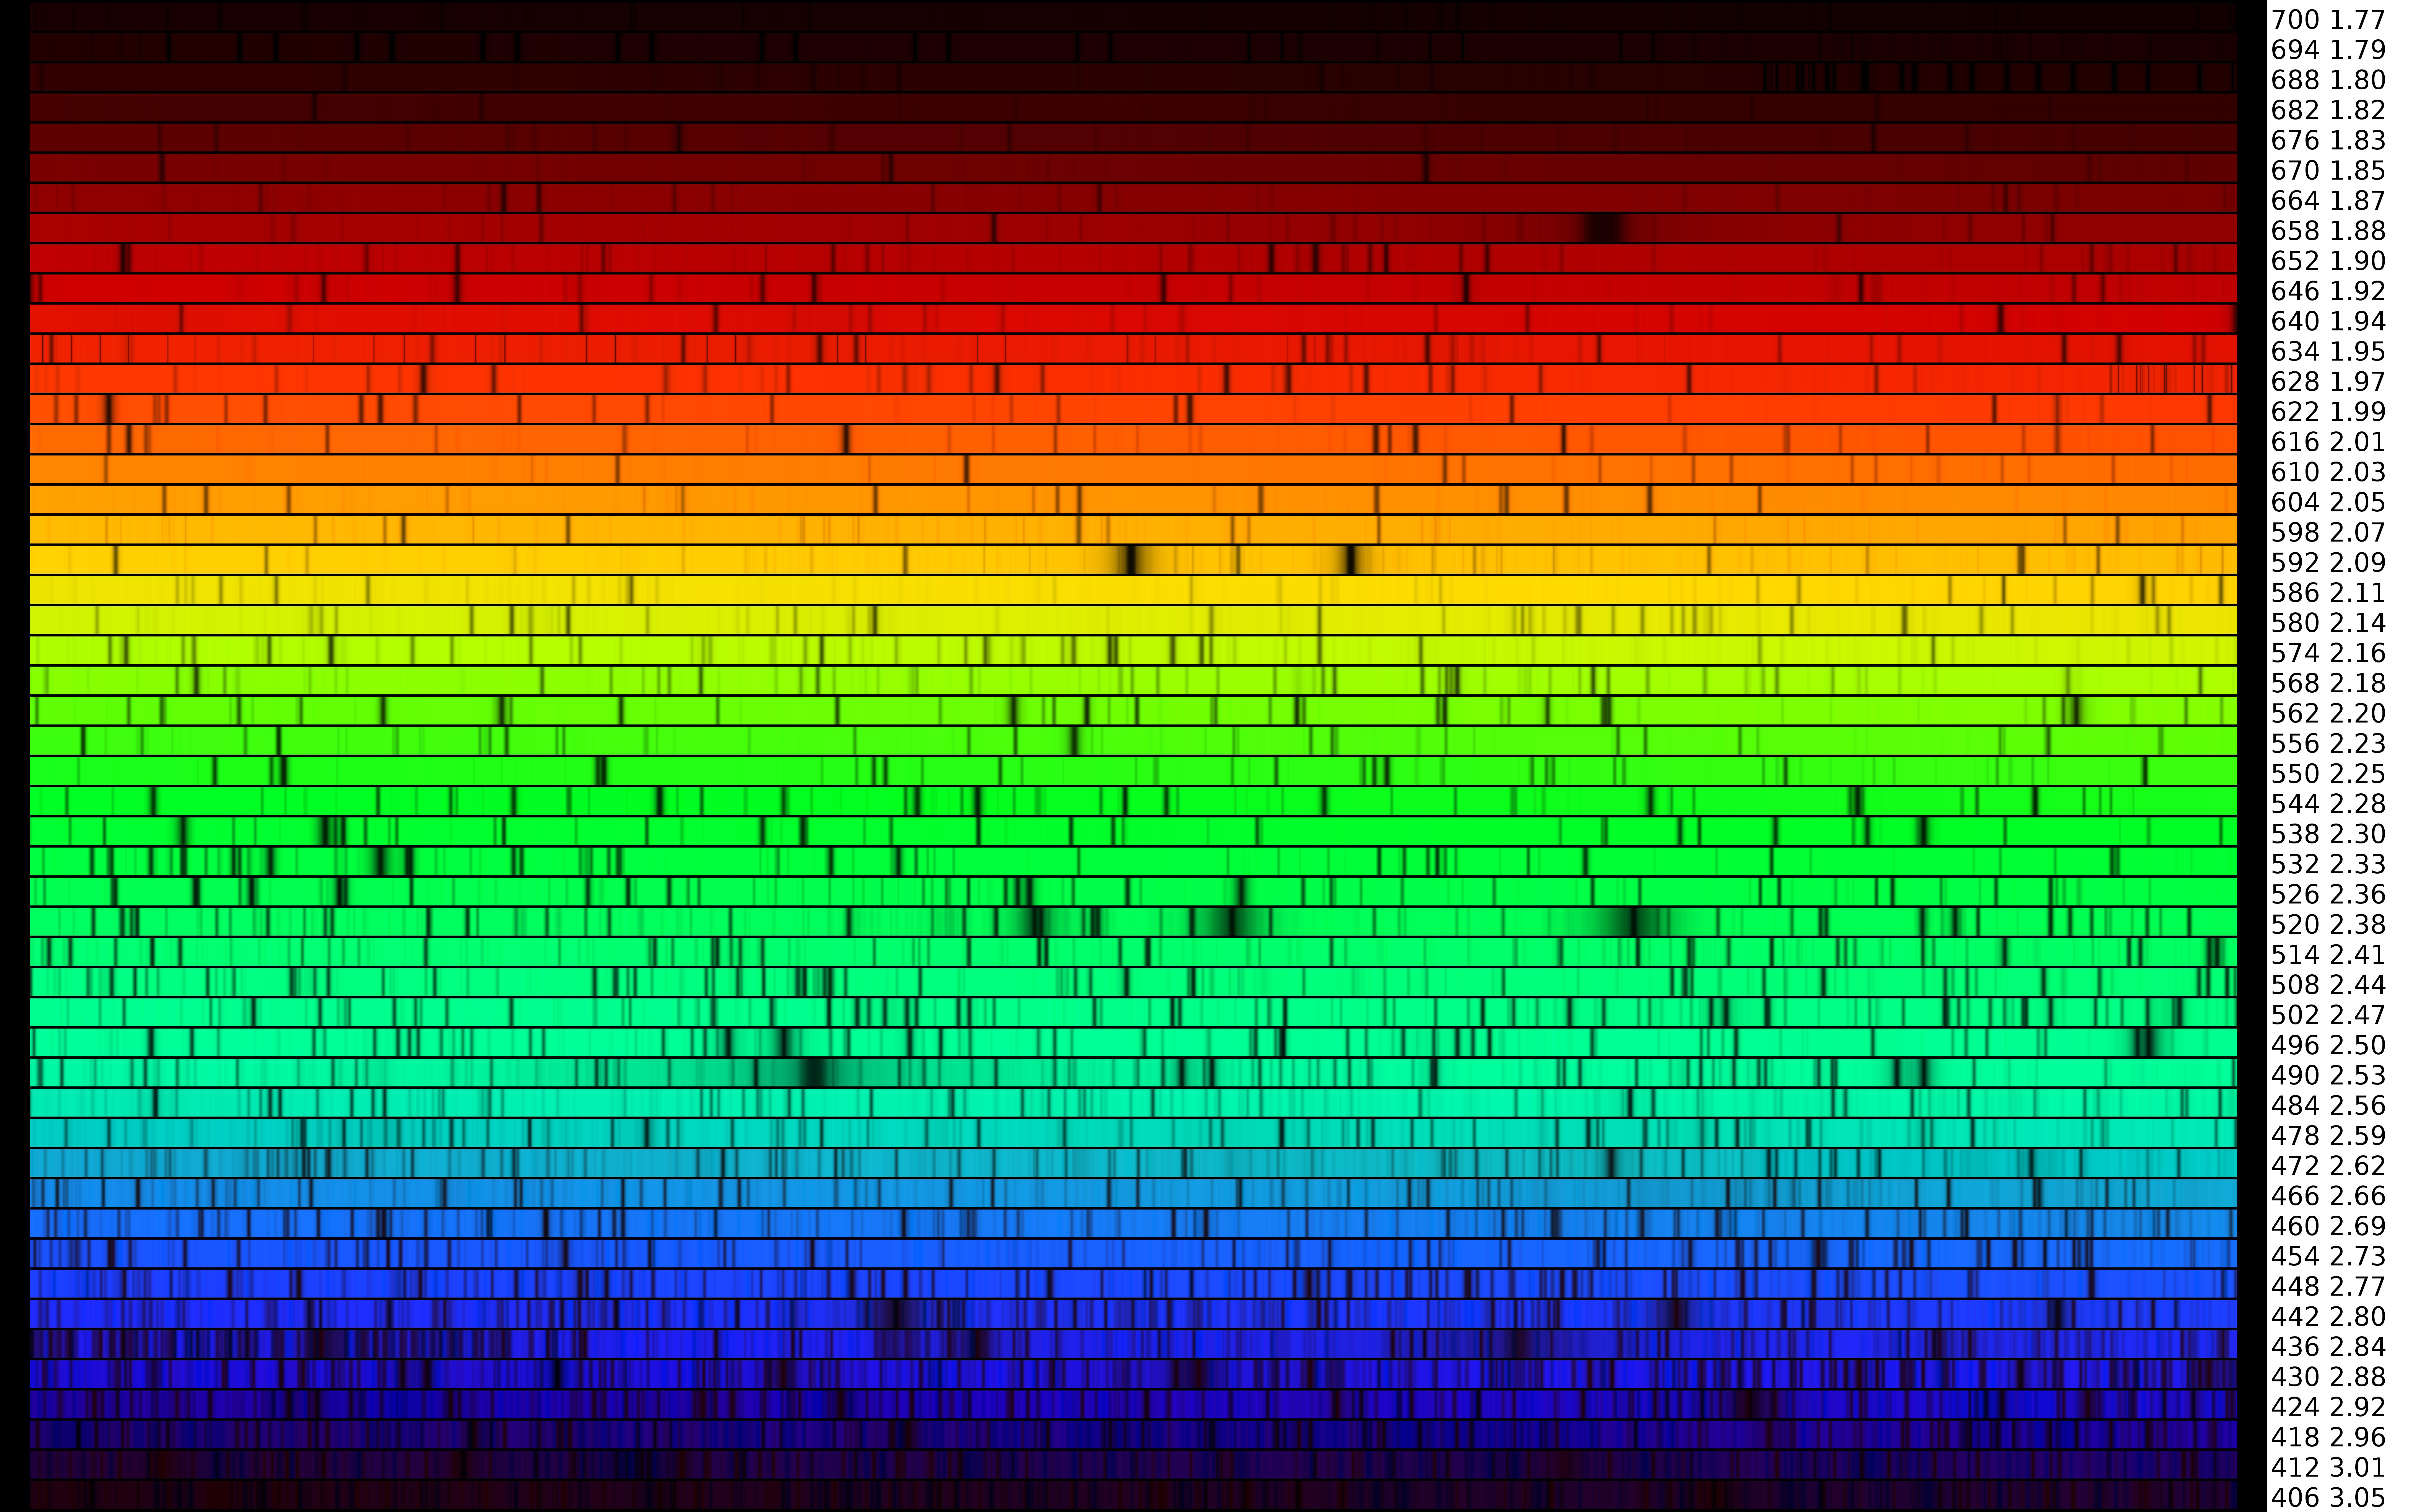
\includegraphics[width=\textwidth]{solarspectrum.jpg}\EC
}

\frame{\frametitle{\textbf{Announcements}}
.
}

\frame{\frametitle{\textbf{Chemistry done ${\rm \bf quick}^{\dagger}$}}

A wave in empty space can have any frequency/wavelength it likes, as we learned Tuesday.

\BS

But a {\it confined} wave can have only very particular frequencies -- the resonant frequencies of the box you put it in.

\BS

Quantum mechanics says that electrons have wave properties, and that frequency corresponds to energy!

\BI
\item In an atom, the electric force confines the electron-waves to a region near the nucleus
(I can't show you this)
\pause
\item In a drum, the frame of the drum confines the drumhead-waves to a circular cavity. I {\bf can} show you this!
\item The shape is different, but there is a close analogy here:
\item {\color{Red} The different wave-shapes in a drum correspond to the different atomic energy levels in chemistry!}
\EI
}

\frame{\frametitle{\textbf{Chemistry done ${\rm \bf quick}^{\dagger}$}}
A remarkable consequence of quantum mechanics:

\BC
\large
Electrons in an atom can only have {\bf very particular} amounts of energy!

\BS\BS

These energy levels correspond to the resonant frequencies of the ``box'' they're trapped in.

\BS\BS

We measure this energy in ``electron volts'' (eV).

\EC

\BI
\item Usually all the electrons live in the lowest available levels
\item There's a limit to how many electrons can be in each level
\item Atoms ``fill up'' the levels starting from the bottom
\item This process leads to the periodic table
\EI
\pause
\begin{flushright}\scriptsize $\dagger$ Does not replace your introductory chemistry class on your transcript\end{flushright}
}

\frame{\frametitle{\textbf{Chemistry done ${\rm \bf quick}^{\dagger}$}}

\BI
\item As in the drum, the energy levels in atoms are controlled by two numbers:
\BI
\item ``Inside-to-outside wiggliness'': {\bf principal quantum number} $n$
\item ``Around-and-around wiggliness'': {\bf angular quantum number} $l$
\EI
\pause
\item Chemists call $l=0$ the S-orbitals, $l=1$ the P-orbitals,
$l=2$ the D-orbitals, and so on.

\BS\BS

\item In hydrogen, the value of $l$ doesn't affect the energy much at all.
\item In other elements, it does a little bit.
\EI
}

{
\setbeamercolor{background canvas}{bg=white}
\frame{\frametitle{\bf Hydrogen}
\color{Black}
\BC Here's a diagram of the allowed energies for hydrogen. 

\BS
\BS

\includegraphics[width=0.6\textwidth]{h1-crop.pdf}
\EC
}
}

\frame{\frametitle{\bf Chemistry: all I want you to know}
\large
\BI
\item Electrons occupy certain {\bf energy levels}
\item The particular energies that these levels have is {\bf unique} to particular elements: hydrogen has different allowed energies than mercury or neon or sodium etc.
\EI

\BS
\BS
\BC ... that's it. :) 
\EC
}

{
\setbeamercolor{background canvas}{bg=white}

\frame{\frametitle{\bf Chemistry and light}
\color{Black}

\BC
\large
How do electrons get to different energy levels?

\BS

\BI
\color{Black}
\item They can {\it absorb} a photon and move to a higher energy level
\item They can {\it emit} a photon and move to a lower energy level
\EI
\BS
\includegraphics[width=0.6\textwidth]{h1-crop.pdf}
\EC
}


\frame{\frametitle{\bf Chemistry and light}
\color{Black}

\BC
\large

\BS

\BI
\color{Black}
\item They can {\it absorb} a photon and move to a higher energy level
\item They can {\it emit} a photon and move to a lower energy level
\EI

\BS

Absorb a 12.1 eV photon and move from $n=1$ to $n=3$; this photon is UV.

\BS
\includegraphics[width=0.6\textwidth]{h2-crop.pdf}
\EC
}

\frame{\frametitle{\bf Chemistry and light}
\color{Black}

\BC
\large

\BS

\BI
\color{Black}
\item They can {\it absorb} a photon and move to a higher energy level
\item They can {\it emit} a photon and move to a lower energy level
\EI

\BS

Emit a 1.9 eV photon and move from $n=3$ to $n=2$. {\color{Red}This is red!}

\BS
\includegraphics[width=0.6\textwidth]{h3-crop.pdf}
\EC
}

\frame{\frametitle{\bf Chemistry and light}
\color{Black}

\BC
\large

\BS

\BI
\color{Black}
\item They can {\it absorb} a photon and move to a higher energy level
\item They can {\it emit} a photon and move to a lower energy level
\EI

\BS

Emit a 10.2 eV photon and move from $n=2$ to $n=1$. (UV, again)

\BS
\includegraphics[width=0.6\textwidth]{h4-crop.pdf}
\EC
}
}
\frame{


If I take hydrogen and tear the electrons off of the atoms with an electric current,
they'll ``fall'' back down, going through the energy levels down to $n=1$.

\BS

Sometimes they'll skip energy levels; sometimes they'll go in sequence.

\BS

If I do this to hydrogen, what color will we see?

\BS
\BS

\color{A}A: UV: we won't see it, since the transitions down to $n=1$ are in the UV\\

\BS

\color{B}B: Several shades of red: we'll see the transitions down to $n=2$, which are red\\ 

\BS

\color{C}C: Infrared: the transitions at the top are very low energy, corresponding to
infrared light which we can't see \\ 

\BS

\color{D}D: UV, IR, and red, all at once: all the transitions happen, but we only see the
red photons because of the limits of our eyes\\ 

\BS

\pause

\color{E}E: Orange, because this is Syracuse, darnit! 
}

\frame{
\Large
\BC
Complete {\it Lecture Tutorials} pp.65-69.

\BS
\BS
\normalsize
After this, we'll talk about another application of this idea.
\EC}

\frame{\frametitle{\bf Emission spectra}

\large

Every chemical element has a unique {\it spectrum}: the colors of light that it can emit and absorb.

\BS

Other colors simply pass through.

\BS

(Molecules have these spectra too: their electron energy levels are more complicated.)

}


\frame{

\BC
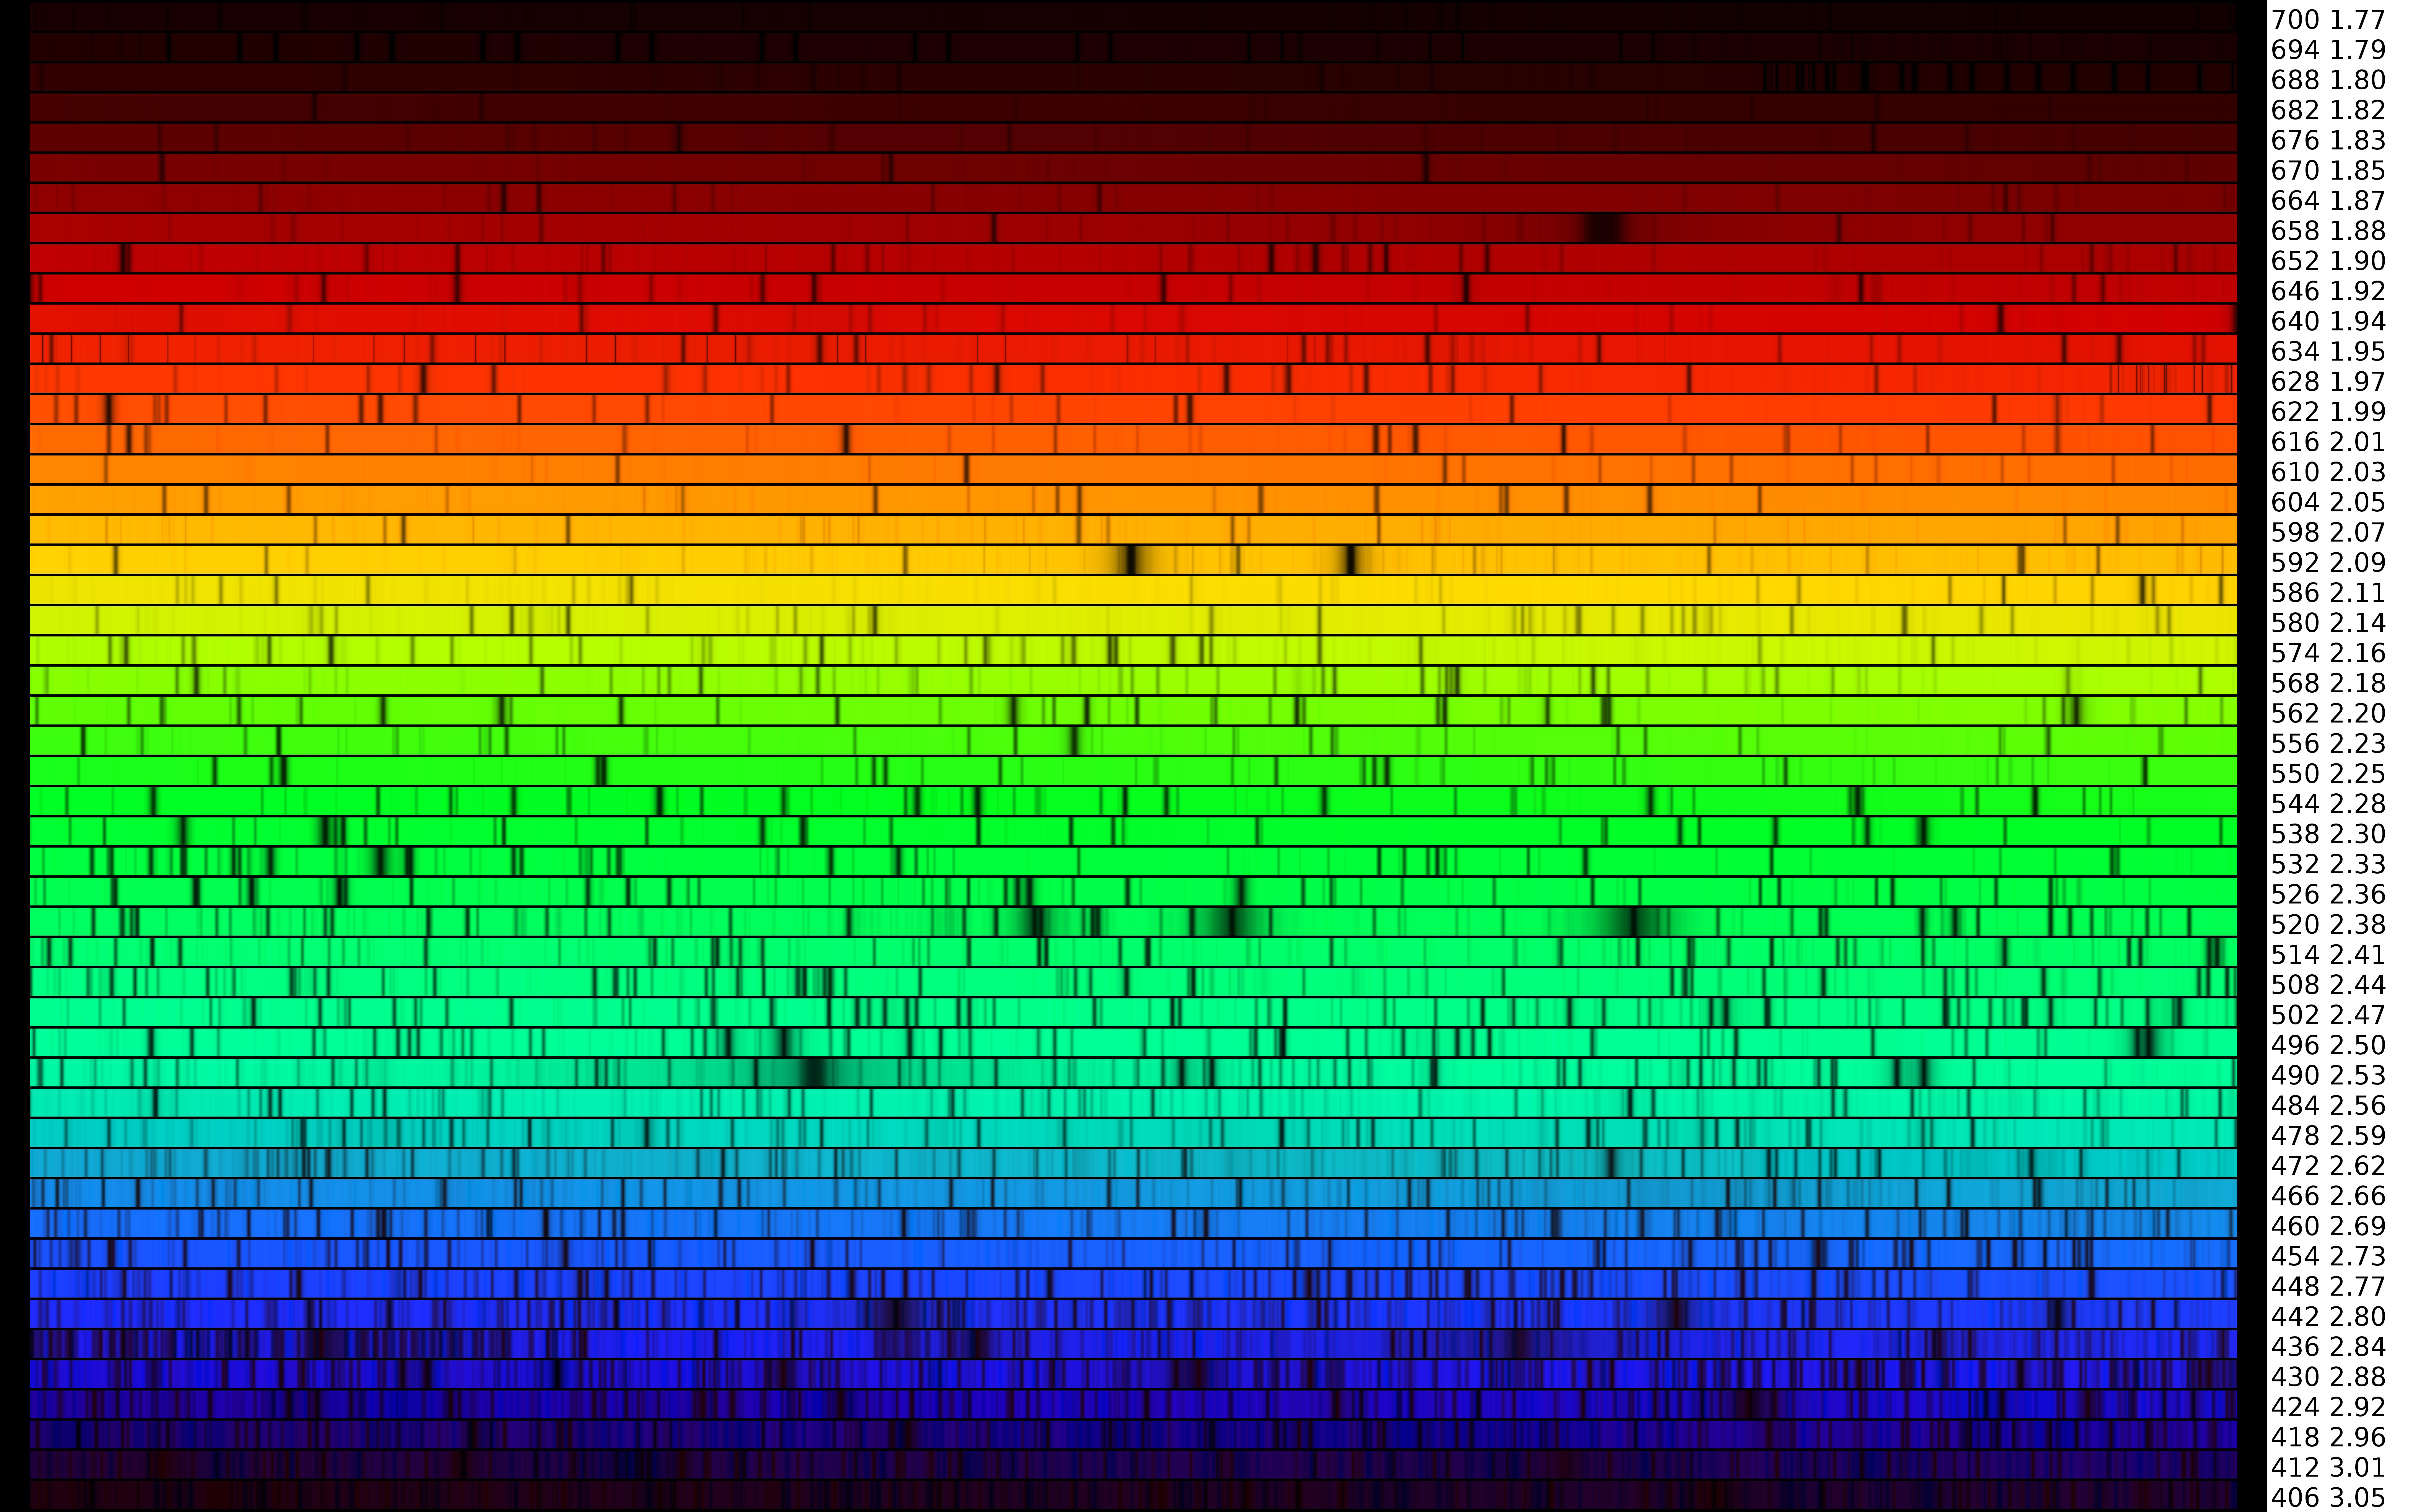
\includegraphics[width=0.7\textwidth]{solarspectrum.jpg}
\EC

\BI
\item The hot core of the Sun emits light of all wavelengths (you'll learn why next class)
\pause
\item The gases in the cooler atmosphere absorb light of their particular wavelengths
\pause
\EI
\BC
\color{Red} \large This picture tells us what's in the Sun!
\EC
}

\frame{

\Large

You discover lines in the solar spectrum that don't correspond to any known element.
What do you conclude?

\BS

\color{A}A: Something about quantum mechanics is different in the Sun\\\BS

\color{B}B: Something about light is different in the Sun\\\BS
\color{C}C: There's an element in the Sun that's not on Earth -- call it {\bf sunium} \\ \BS
\color{D}D: The extreme temperature of the Sun causes new lines to appear in its gas \\
}


\frame{

\BC
\includegraphics[width=0.95\textwidth]{stellar-spectra.jpg}
\BS

\large

All the stars are made of the same stuff -- the same stuff as we are.\pause
\EC
``The cosmos is also within us. We are made of star-stuff. We are a way for the universe to know itself.''

\begin{flushright}--Carl Sagan, {\it Cosmos} \end{flushright}
}

\frame{\frametitle{\textbf What a lucky accident!}
\large 
We're very lucky that atomic transitions happen to lie in our visual range!

There are others that are very interesting to astronomers:

\BI
\item Molecular vibrations: infrared
\pause
\item Molecular {\it rotations}: microwave
\pause
\item ``Hyperfine structure'' energy levels in hydrogen: 21 cm radio waves
\EI

\pause

\normalsize

This last is particularly interesting: it is a very particular frequency, echoing out from
all corners of the Universe, that says: hydrogen is here. (Hydrogen is 75\% of the universe.)
}

\frame{
\BC
\includegraphics[width=0.5\textwidth]{pioneer-10.jpg}
\EC
}

\frame{
\BC
\includegraphics[width=0.8\textwidth]{pioneer-plaque.jpg}
\EC
}

\frame{
\BC
\includegraphics[width=0.7\textwidth]{pioneer-plaque-2.jpg}\\
\includegraphics[width=0.3\textwidth]{hyperfine.jpg}
\EC
}

\end{document}

